

\documentclass[final]{cvpr}

\usepackage{times}
\usepackage{epsfig}
\usepackage{graphicx}
\usepackage{amsmath}
\usepackage{amssymb}

\usepackage{subcaption}
\usepackage{caption}
\usepackage{multirow}
\usepackage{tabularx}
\usepackage[symbol]{footmisc}
\usepackage{verbatim}


\makeatletter
\@namedef{ver@everyshi.sty}{}
\makeatother
\usepackage{tikz}
\usepackage{pgfplots}
\usepackage{pgfplots}\pgfplotsset{compat=1.9}

\newcommand*{\affaddr}[1]{#1} \newcommand*{\affmark}[1][*]{\textsuperscript{#1}}
\newcommand*{\email}[1]{#1}
\renewcommand{\thefootnote}{\fnsymbol{footnote}}




\usepackage[pagebackref=true,breaklinks=true,colorlinks,bookmarks=false]{hyperref}


\def\cvprPaperID{6983} \def\confYear{CVPR 2021}



\begin{document}

\title{GAN Prior Embedded Network for Blind Face Restoration in the Wild}



\author{Tao Yang\affmark[1], Peiran Ren\affmark[1], Xuansong Xie\affmark[1], and Lei Zhang\affmark[1,2]\footnotemark\\
\affaddr{\affmark[1]DAMO Academy, Alibaba Group}\\
\affaddr{\affmark[2]Department of Computing, The Hong Kong Polytechnic University}\\
\email{\tt\small{yangtao9009@gmail.com, peiran\_r@sohu.com, xingtong.xxs@taobao.com, cslzhang@comp.polyu.edu.hk}}\\
}

\maketitle


\begin{abstract}
Blind face restoration (BFR) from severely degraded face images in the wild is a very challenging problem. Due to the high illness of the problem and the complex unknown degradation, directly training a deep neural network (DNN) usually cannot lead to acceptable results. Existing generative adversarial network (GAN) based methods can produce better results but tend to generate over-smoothed restorations. In this work, we propose a new method by first learning a GAN for high-quality face image generation and embedding it into a U-shaped DNN as a prior decoder, then fine-tuning the GAN prior embedded DNN with a set of synthesized low-quality face images. The GAN blocks are designed to ensure that the latent code and noise input to the GAN can be respectively generated from the deep and shallow features of the DNN, controlling the global face structure, local face details and background of the reconstructed image. The proposed GAN prior embedded network (GPEN) is easy-to-implement, and it can generate visually photo-realistic results. Our experiments demonstrated that the proposed GPEN achieves significantly superior results to state-of-the-art BFR methods both quantitatively and qualitatively, especially for the restoration of severely degraded face images in the wild. The source code and models can be found at \url{https://github.com/yangxy/GPEN}. 
\end{abstract}

\section{Introduction}
\footnotetext[1]{This work is partially supported by the Hong Kong RGC RIF grant (R5001-18).}


























Face images are among the most popular types of images in our daily life, while face images are often degraded due to the many factors such as low resolution, blur, noise, compression, etc., or the combination of them. Face image restoration has been attracting significant attentions, aiming at reproducing a clear and realistic face image from the degraded input. Traditional face image restoration methods \cite{Zhang2011Sparseprior,Bourlai2011Restore,Bakerand2000Hallucinate,Nishiyama2009Face} usually solve an inverse problem based on the degradation model and handcrafted priors, which demonstrate limited performance in practice. Recently, deep neural networks (DNNs) have shown superior results in a variety of computer vision tasks \cite{Kupyn2017DeblurGAN,Yu2018Deepfill,Guo2019CBDNet,Ledig2017SRGAN,Lim2017EDSR}, and many DNN based face restoration methods \cite{Yu2017Hallucinating,Li2018GFRNet,Hu20203dprior} have also been developed and they have demonstrated much better performance than traditional ones. 

Though much progress has been made for face restoration, blind face restoration (BFR) remains a challenging research problem because of the unknown and complex degradation of low quality (LQ) face images in the wild. In order to recover a high-quality (HQ) face image with photo-realistic textures from an LQ face image, a number of BFR methods have been proposed by resorting to the spatial transformer networks \cite{Yu2017Hallucinating}, exemplar images \cite{Li2018GFRNet,Li2020ASFFNet,Dogan2019Exemplar}, 3D facial priors \cite{Hu20203dprior}, and facial component dictionaries \cite{Li2020Restore}. Yang \emph{et al}. \cite{Yang2020HiFaceGANFR} proposed a collaborative suppression and replenishment (CSR) approach to progressively replenish facial details. These methods exhibit impressive results on artificially degraded faces; however, they fail to tackle real-world LQ face images. The conditional generative adversarial network (cGAN) based methods such as Pix2Pix \cite{Isola2017Pix2Pix} and Pix2PixHD \cite{Wang2018Pix2PixHD} learn a direct mapping from input image to output image. These methods achieve more realistic results but tend to over-smooth the images (see Figures~\ref{fig:comp} and \ref{fig:realcomp}), which is commonly blamed to the high illness of real-world BFR tasks. 

With the rapid advancement of GAN techniques \cite{Karras2018StyleGAN,Karras2019StyleGAN2}, recently some methods have been proposed to reconstruct faces from extremely low resolution inputs \cite{Gu2019Prior,Menon2020PULSE,Richardson2020pSp}. Richardson \emph{et al}. \cite{Richardson2020pSp} employed an encoder network to generate a series of style vectors before feeding them into a pre-trained generator, achieving a generic image-to-image translation framework. However, such methods can only work on non-blind image super-resolution problems. Furthermore, they kept the pre-trained GAN unchanged in training for the consistency and convenience of face manipulations. This however leads to unstable quality of restored faces when dealing with real-world LQ face images with complex background, because it is hard to accurately project a face image with limited resolution to a desired latent code (e.g., a vector of size  in StyleGAN \cite{Karras2018StyleGAN,Karras2019StyleGAN2}).

In this work, we revisit the problem of BFR and target at restoring HQ faces from degraded face observations in the wild. Our idea is to seamlessly integrate the advantages of GAN and DNN. We first pre-train a GAN for HQ face image generation and embed it into a DNN as a decoder prior for face restoration. The GAN prior embedded DNN is then fine-tuned by a set of synthesized LQ-HQ face image pairs, during which the DNN learns to map the input degraded image to a desired latent space so that the GAN prior network can reproduce the desired HQ face images. We carefully design the GAN blocks to make them well suited for a U-shaped DNN, where the deep features are used to generate the latent code for global face reproduction, while the shallow features are used as noise to generate local face details and keep the image background. In this way, our learned model can reconstruct HQ faces with photo-realistic details from even severely degraded face images in the wild, avoiding over-smoothed results caused by the high illness of the BFR problem. Figure~\ref{fig:oldphotos} shows an example. One can see that our model reconstructs the face images of those great scientists with clear details from the old photo taken in 1927. 

\vspace*{2mm}
The main contributions of this work are summarized as follows:
\vspace*{-2mm}
\begin{itemize}
  \setlength{\itemsep}{0.7pt}
  \setlength{\parsep}{0.7pt}
  \setlength{\parskip}{0.7pt}
\item We learn and embed a GAN prior network into a DNN, and fine-tune the GAN embedded DNN for effective BFR in the wild. It is worthy to note that previous works only transfer the pre-trained GAN into a network without fine-tuning.
   \item The GAN blocks are designed so that they can be easily embedded into a U-shaped DNN for fine-tuning. The latent code and noise input of the GAN are respectively generated from the deep and shallow features of the DNN to reconstruct the global structure, local face details and background of the image accordingly.
   \item Our model sets new state-of-the-art in BFR. It is capable of tackling severely degraded face images taken in real-world scenarios.
\end{itemize}
\vspace*{-2mm}

\begin{figure}
   \includegraphics[width=.5\textwidth]{imgs/oldphoto-compressed.pdf}
   \caption{Restored face images from the group photo taken in the Solvay Conference, 1927. Best viewed by zooming to  in the screen.}
\label{fig:oldphotos}
\vspace*{-5mm}
\end{figure}

\section{Related Work}


\textbf{Face Image Restoration.}
As a specific but important branch of image restoration, face image restoration has been widely studied for many years. In the early stage, Zhang \emph{et al}. \cite{Zhang2011Sparseprior} presented a joint blind image restoration and recognition method by using sparse representation to handle face recognition from LQ images. Nishiyama \emph{et al}. \cite{Nishiyama2009Face} proposed to improve the recognition performance of blurry faces by using a pre-defined set of blur kernels to restore them. With the unprecedented success of DNNs in solving image restoration tasks such as denoising \cite{Guo2019CBDNet}, deblurring \cite{Kupyn2017DeblurGAN,Shen2018Deblur}, inpainting \cite{Yu2018Deepfill,Liu2018Partialconv} and image super-resolution \cite{Ledig2017SRGAN,Lim2017EDSR}, many DNN based face image restoration methods have also been proposed \cite{Chen2018FSRNet,Kim2019PFSR,Ma2020FSR}, which advance the traditional methods by a large margin. Considering the fact that facial images have specific structures, it is interesting to investigate whether we can restore a clear face image from severely degraded ones without knowing the degradation model. The so-called blind face restoration (BFR) problem has been attracting intensive research attentions in recent years \cite{Li2018GFRNet,Dogan2019Exemplar,Li2020Restore,Yang2020HiFaceGANFR}, while it is still a challenging task due to the complex image degradations in the wild.

Huang \emph{et al}. \cite{Huang2017Wavelet} presented a wavelet-based approach that can ultra-resolve a very low-resolution (LR) face image. Chen \emph{et al}. \cite{Chen2018FSRNet} learned the facial geometry prior to recover the high-resolution (HR) faces. Ma \emph{et al}. \cite{Ma2020FSR} performed face super-resolution with iterative collaboration between two recurrent networks on facial image recovery and landmark estimation, respectively. Li \emph{et al}. \cite{Li2018GFRNet} used a guiding image and a wrapper subnetwork to cope with appearance variations between the LR input and the HR guiding image. This work was further extended by using an unconstrained HR face image \cite{Dogan2019Exemplar}, multi-exemplar images \cite{Li2020ASFFNet}, and multi-scale component dictionaries \cite{Li2020Restore}. Hu \emph{et al}. \cite{Hu20203dprior} explicitly incorporated 3D facial priors to grasp the sharp facial structures. A collaborative suppression and replenishment approach was proposed by Yang \emph{et al}. \cite{Yang2020HiFaceGANFR} to progressively replenish facial details. Existing works have generated impressive results on artificially degraded faces, but often failed in real-world scenarios due to the complex unknown degradation. Furthermore, their performance depends heavily on the accurate facial prior knowledge which however is hard to obtain from severely degraded face images in the wild, leading to unpredictable failures.







\textbf{Generative Adversarial Network (GAN).}
Since the seminal work by Goodfellow \emph{et al}. \cite{Goodfellow2014GAN}, great progress has been accomplished on learning GAN models \cite{Karras2018PGGAN,Brock2019BigGAN,Karras2018StyleGAN,Karras2019StyleGAN2}. GAN has been widely used for various computer vision applications due to its powerful ability to generate photo-realistic images. Some typical applications include image inpainting \cite{Yu2018Deepfill}, super-resolution \cite{Ledig2017SRGAN,Wang2018ESRGAN}, image colorization \cite{Isola2017Pix2Pix,Suarez2017Color}, texture synthesis \cite{Slossberg2018Texture}, etc. Particularly, to provide more user controls for image synthesis, conditional GAN (cGAN) has been proposed \cite{Mirza2014cGAN}. By feeding the generator with different conditional information \cite{Park2019SPADE,Isola2017Pix2Pix,Zhu2017CycleGAN}, cGANs succeed in handling various image-to-image translation problems. Isola \emph{et al}. \cite{Isola2017Pix2Pix} showed that the conditional adversarial networks can be used as a general-purpose solution to image-to-image translation problems. Many following works, such as unsupervised learning \cite{Zhu2017CycleGAN}, disentangled learning \cite{Lee2018DRIT}, few-shot learning \cite{Liu2019Few}, high resolution image synthesis \cite{Wang2018Pix2PixHD}, multi-domain translation \cite{Choi2018Stargan}, multi-modal translation \cite{Zhu2017Multimodal}, have been proposed to extend cGAN to different scenarios. The cGAN learns a direct mapping from the input domain to the output one. Unfortunately, the generated results by cGANs are usually over-smoothed in highly ill-posed tasks such as BFR.


\textbf{GAN Prior for Image Generation.}
Deep generative models are popular in solving many inverse problems, e.g. deblurring \cite{Kupyn2017DeblurGAN}, image inpainting \cite{Yu2018Deepfill}, phase retrieval \cite{Hand2018Phase}, etc. Recently, many works have been developed for the task of GAN inversion, i.e., reversing a given image back to a latent code with a pre-trained GAN model. Existing methods either optimize the latent code \cite{Abdal2019Img2StyleGAN} or learn an extra encoder to project the image space back to the latent space \cite{Gu2019Prior,Richardson2020pSp}. Abdal \emph{et al}. \cite{Abdal2019Img2StyleGAN} embedded images into an extended latent space of StyleGAN, allowing further semantic image editing operations. Gu \emph{et al}. \cite{Gu2019Prior} employed multiple latent codes to generate multiple feature maps to output the final image. These optimization-based methods, however, are slow and improper for real-world applications. To address this issue, Pixel2Style2Pixel (pSp) \cite{Richardson2020pSp} embeds real images into extended latent space without additional optimization, which can be used in a wide range of image-to-image translation tasks. Menon \emph{et al}. \cite{Menon2020PULSE} proposed a self-supervised approach that traverses the HR natural image manifold, searching for images that can downscale to the original LR image. GAN inversion is an important step for applying GANs to real-world applications. However, it is difficult to perfectly project the image space back to the latent space. Moreover, it is hard, if not possible, to invert a blindly degraded face into a latent space.

Some works were proposed to transfer GAN priors. Wang \emph{et al}. \cite{Wang2018TransferGAN} applied domain adaptation to image generation with
GANs. They further proposed a novel knowledge transfer method for generative models by using a knowledge mining network \cite{Wang2020MineGAN}. Fr{\'e}gier and Gouray \cite{Frgier2019Mind2MindT} introduced a novel approach for transfer learning with GAN architecture. These works target at transferring the knowledge from the source domain to different target domains, while in our work, the source and target domains are the same. We embed the GAN prior learned for face generation into a DNN for face restoration, and jointly fine-tune the GAN prior network with the DNN so that the latent code and noise input can be well generated from the degraded face image at different network layers.









\begin{figure}[t!]
\centering
\includegraphics[width=0.48\textwidth]{imgs/motivation.pdf}
\caption{Illustration of the motivation and framework of our GAN prior embedded network (GPEN).}
\label{fig:motivation}
\vspace*{-3mm}
\end{figure}

\begin{figure*}[t!]
\centering
\includegraphics[width=0.96\textwidth]{imgs/architecture.pdf}
\caption{The architecture of GPEN. (a) The GAN prior network; (b) detailed structures of a GAN block; and (c) the full network architecture of GPEN. The definition of ``Mod'' and ``Demod'' can be found in \cite{Karras2019StyleGAN2}.}
\label{fig:arch}
\vspace*{-3mm}
\end{figure*}

\section{Proposed Method}
\label{sec:proposed}


\subsection{Motivation and Framework}
\label{sec:motivation}
BFR is a typical ill-posed inverse problem. Denote by  the space of degraded LQ faces, and by  the space of original HQ face images. Given an input LQ face image , BFR aims to find its corresponding clear face image . Most of the DNN based methods learn a mapping function  to achieve this goal, i.e., . However, this is a one-to-many inverse problem, and there are many possible face images (e.g., ) in  that can match to the input . Existing methods \cite{Bulat2018SuperFAN,Li2018GFRNet,Dogan2019Exemplar} usually train DNNs to perform mapping between  and  using some pixel-wise loss functions. As a result, as we illustrated in Figure~\ref{fig:motivation}, the final solution  tends to be the mean of those HQ faces, which is over-smoothed and loses details. This coincides with the visual perception global-first theory \cite{Chen2005Global}. The cGAN methods \cite{Isola2017Pix2Pix,Wang2018Pix2PixHD} can partially dilute this issue by adversarial training to reduce the uncertainty in mapping. However, when the degradation is severe, the problem remains and cGANs can hardly generate clear face images with realistic textures and details (see Figure~\ref{fig:comp} for example).

Different from previous methods \cite{Bulat2018SuperFAN,Li2018GFRNet,Dogan2019Exemplar,Wang2018Pix2PixHD,Yang2020HiFaceGANFR}, we first train a GAN prior network, and then embed it into a DNN as decoder for HQ face image restoration. We call our method GAN prior embedded network (GPEN). As illustrated in Figure~\ref{fig:motivation}, the first part of our GPEN is a CNN encoder, which learns to map the input degraded image  to a desired latent code  in the latent space  of the GAN. The GAN prior network can then reproduce the desired HQ face image via , where G refers to the learned generator of GAN. The generation process is basically a one-to-one mapping, largely alleviating the uncertainty of one-to-many mapping in previous methods. It should be noted that the GAN inversion methods \cite{Gu2019Prior,Menon2020PULSE,Richardson2020pSp} share a similar idea with our GPEN; however, they keep the pre-trained GANs unchanged for consistent and convenient face manipulations. While in GPEN, we carefully design and pre-train the GAN blocks and fine-tune the GAN priors for effective BFR. The architectures of GPEN and GAN blocks are shown in Figure~\ref{fig:arch} and will be explained in detail in the following sections.

















\subsection{Network Architecture}
\label{sec:model}
\textbf{The GAN prior network.}
U-Net \cite{Ronneberger2015Unet} has been successfully and widely used in many image restoration tasks \cite{Wang2018Pix2PixHD,Guo2019CBDNet} and demonstrated its effectiveness in preserving image details. Therefore, our GPEN overall follows a U-shaped encoder-decoder architecture (see Figure~\ref{fig:arch}(c)). Accordingly, the GAN prior network should be designed to meet two requirements: 1) it is capable of generating HQ face images; and 2) it can be readily embedded into the U-shaped GPEN as a decoder. Inspired by the state-of-the-art GAN architectures, e.g., StyleGAN \cite{Karras2018StyleGAN,Karras2019StyleGAN2}, we use a mapping network to project latent code  into a less entangled space , as illustrated in Figure~\ref{fig:arch}(a). The intermediate code  is then broadcasted to each GAN block. Since the GAN prior network will be embedded into a U-shaped DNN for finetuning, we need to leave room for the skipped feature maps extracted by the encoder of the U-shaped DNN. We thus provide additional noise inputs to each GAN block. 

For the structure of GAN block, there are several options. In this work, we adopt the architecture in StyleGAN v2 (see Figure~\ref{fig:arch}(b)) due to its high capability to generate HQ images. (Alternative GAN architectures such as StyleGAN v1 \cite{Karras2018StyleGAN}, PGGAN \cite{Karras2018PGGAN} and BigGAN \cite{Brock2019BigGAN} can also be easily adopted into our GPEN.) The number of GAN blocks is equal to the number of skipped feature maps extracted in the U-shaped DNN (and the number of noise inputs), which is related to the resolution of input face image. StyleGAN requires two different noise inputs in each GAN block. To enable the GAN prior network to be readily embedded into the U-shaped GPEN, different from StyleGAN, the noise inputs are reused at the same spatial resolution for all GAN blocks. Furthermore, the noise inputs are concatenated rather than added to the convolutions in StyleGAN. We empirically found that this can bring more details in the restored face image.









\textbf{Full network architecture.}
Once the GAN prior network is trained by using some dataset (e.g., the FFHQ \cite{Karras2018StyleGAN} dataset), we embed it into the U-shaped DNN as a decoder, as shown in Figure~\ref{fig:arch}(c). The latent code  and the noise inputs to the GAN network are replaced by the output of the fully-connected layer (i.e., deeper features) and shallower layers of the encoder of the DNN, respectively, which will control the reconstruction of global face structure, local face details, as well as the background of face image. Since the proposed model is not fully convolutional, LQ face images are first resized to the desired resolution (e.g., ) using simple bilinear interpolator before being input to the GPEN. After embedding, the whole GPEN will be fine-tuned so that the encoder part and decoder part can learn to adapt to each other. 







\subsection{Training Strategy}
\label{sec:training}
We first pre-train the GAN prior network using a dataset of HQ face images following the training strategies of StyleGAN \cite{Karras2018StyleGAN,Karras2019StyleGAN2}. The pre-trained GAN model is embedded into the proposed GPEN, and we fine-tune the whole network using a set of synthesized LQ-HQ face image pairs (the image synthesis process will be given in Section~\ref{sec:degradation}).  

To fine-tune the GPEN model, we adopt three loss functions: the adversarial loss , the content loss , and the feature matching loss .  is inherited from the GAN prior network:

where  and  denote the ground-truth HQ image and the degraded LQ one,  is the generator during training, and  is the discriminator.  is defined as the -norm distance between the final results of the generator and the corresponding ground-truth images.  is similar to the perceptual loss \cite{Johnson2016Perceptual} but it is based on the discriminator rather than the pre-trained VGG network to fit our task. It is formulated as follows:

where  is the total number of intermediate layers used for feature extraction.  is the extracted feature at the -th layer of discriminator . 

The final loss  is as follows:

where  and  are balancing parameters. The content loss  enforces the fine features and preserves the original color information. By introducing the feature matching loss  on the discriminator, the adversarial loss  can be better balanced to recover more realistic face images with vivid details. In all the following experiments, we empirically set  and .

























\section{Experiments}
\label{sec:experiments}
\subsection{Datasets and Evaluation Metric}
The FFHQ dataset \cite{Karras2018StyleGAN}, which contains  HQ face images of resolution , is used to train our GPEN model. We first use it to train the GAN prior network, and then synthesize LQ images from it to fine-tune the whole GPEN. To evaluate our model, we use the CelebA-HQ dataset \cite{Karras2018PGGAN} to simulate LQ face images to quantitatively compare GPEN with other state-of-the-art methods. We also collet  real-world LQ faces (will be made publicly available) from internet to qualitatively evaluate the performance of our model in the wild. In the quantitative evaluation, the Peak Signal-to-Noise Ratio (PSNR),  the Fr\'echet Inception Distances (FID) \cite{Heusel2017FID} and the Learned Perceptual Image Patch Similarity (LPIPS) \cite{Zhang2018LPIPS} indices are used. It is worth mentioning that all these indices can only be used as references for evaluation because they cannot truly reflect the performance of a BFR method, especially for BFR in the wild. 

\subsection{Implementation Details}
\label{sec:degradation}
We first train the GAN prior network using the FFHQ dataset with similar settings to StyleGAN \cite{Karras2018StyleGAN,Karras2019StyleGAN2}. The pre-trained GAN prior network is embedded into the GPEN to perform fine-tuning. To build LQ-HQ image pairs for fine-tuning, we synthesize degraded faces from the HQ images in FFHQ using the following degradation model:

where , , ,  are respectively the input face image, the blur kernel, the Gaussian noise with standard deviation  and the degraded image. , ,  respectively denote the two-dimensional convolution, the standard -fold downsampler and the JPEG compression operator with a quality factor . 

The above degradation model has been used in previous methods \cite{Li2018GFRNet,Li2020Restore}. In our implementation, for each image the blur kernel  is randomly selected from a set of blurring models, including Gaussian blur and motion blur with varying kernel sizes. The additive Gaussian noise  is sampled channel-wise from a normal distribution, and  is chosen from . The value of  is randomly and uniformly sampled from  (i.e., up to  times downscaling) and  is randomly and uniformly sampled from  (i.e., up to  JPEG compression) per image. By using those severely degraded images to fine-tune the model, the encoder part of our GPEN can learn to generate suitable latent code and noise inputs to the GAN prior decoder network, which is updated simultaneously to tackle severely degraded faces in real-world scenarios. 

During model updating, we adopt the Adam optimizer with a batch size of . The learning rate () varies for different parts of GPEN, including the encoder, the decoder and the discriminator. In our implementation, we let , and set . It should be noted that the discriminator part will be removed in the testing stage. 







\subsection{Ablation Study}
To better understand the roles of different components of GPEN and the training strategy, in this section we conduct an ablation study by introducing some variants of GPEN and comparing their BFR performance. The first variant is denoted by GPEN-w/o-ft, i.e., the embedded GAN prior network is kept unchanged in the fine-tuning process. The second variant is denoted by GPEN-w/o-noise, which refers to the GPEN model without noise inputs. The third variant is denoted by GPEN-noise-add, i.e., that the noise inputs are added rather than concatenated to the convolutions.


\begin{figure*}[ht!]
\centering
\begin{subfigure}[t!]{.16\textwidth}
        \includegraphics[width=\textwidth]{imgs/face/ablation/00116_lr.png}
        \vspace*{-5mm}
        \caption{}
    \end{subfigure} 
    \begin{subfigure}[t!]{.16\textwidth}
        \includegraphics[width=\textwidth]{imgs/face/ablation/00116_wo_ft.png}
        \vspace*{-5mm}
        \caption{}
    \end{subfigure} 
    \begin{subfigure}[t!]{.16\textwidth}
        \includegraphics[width=\textwidth]{imgs/face/ablation/00116_wo_noise.png}
        \vspace*{-5mm}
        \caption{}
    \end{subfigure} 
\begin{subfigure}[t!]{.16\textwidth}
        \includegraphics[width=\textwidth]{imgs/face/ablation/00116_noise_add.png}
        \vspace*{-5mm}
        \caption{}
    \end{subfigure} 
    \begin{subfigure}[t!]{.16\textwidth}
        \includegraphics[width=\textwidth]{imgs/face/ablation/00116_GPEN.png}
        \vspace*{-5mm}
        \caption{}
    \end{subfigure} 
    \begin{subfigure}[t!]{.16\textwidth}
        \includegraphics[width=\textwidth]{imgs/face/ablation/00116_gt.png}
        \vspace*{-5mm}
        \caption{}
    \end{subfigure} 
\vspace*{-3mm}
\caption{Comparisons of our variants BFR. (a) LQ input; (b) GPEN-w/o-ft; (c) GPEN-w/o-noise; (d) GPEN-noise-add; (e) GPEN; (f) Ground truth.} 
\label{fig:ablation}
\vspace*{-3mm}
\end{figure*}

\begin{figure*}[ht!]
\centering
\begin{subfigure}[t!]{.11\textwidth}
        \includegraphics[width=\textwidth]{imgs/face/syn/00800_input.png}
    \end{subfigure}\begin{subfigure}[t!]{.11\textwidth}
        \includegraphics[width=\textwidth]{imgs/face/syn/00800_SuperFAN.png}
    \end{subfigure}\begin{subfigure}[t!]{.11\textwidth}
        \includegraphics[width=\textwidth]{imgs/face/syn/00800_GFRNet.png}
    \end{subfigure}\begin{subfigure}[t!]{.11\textwidth}
        \includegraphics[width=\textwidth]{imgs/face/syn/00800_GWAInet.png}
    \end{subfigure}\begin{subfigure}[t!]{.11\textwidth}
        \includegraphics[width=\textwidth]{imgs/face/syn/00800_pix2pixHD.jpg}
    \end{subfigure}\begin{subfigure}[t!]{.11\textwidth}
        \includegraphics[width=\textwidth]{imgs/face/syn/00800_DFDNet.png}
    \end{subfigure}\begin{subfigure}[t!]{.11\textwidth}
        \includegraphics[width=\textwidth]{imgs/face/syn/00800_HiFaceGAN.jpg}
    \end{subfigure}\begin{subfigure}[t!]{.11\textwidth}
        \includegraphics[width=\textwidth]{imgs/face/syn/00800_ours.png}
    \end{subfigure}\begin{subfigure}[t!]{.11\textwidth}
        \includegraphics[width=\textwidth]{imgs/face/syn/00800_gt.png}
    \end{subfigure}\\
    \begin{subfigure}[t!]{.11\textwidth}
        \includegraphics[width=\textwidth]{imgs/face/syn/00410_input.png}
        \vspace*{-5mm}
        \caption{}
    \end{subfigure}\begin{subfigure}[t!]{.11\textwidth}
        \includegraphics[width=\textwidth]{imgs/face/syn/00410_SuperFAN.png}
        \vspace*{-5mm}
        \caption{}
    \end{subfigure}\begin{subfigure}[t!]{.11\textwidth}
        \includegraphics[width=\textwidth]{imgs/face/syn/00410_GFRNet.png}
        \vspace*{-5mm}
        \caption{}
    \end{subfigure}\begin{subfigure}[t!]{.11\textwidth}
        \includegraphics[width=\textwidth]{imgs/face/syn/00410_GWAInet.png}
        \vspace*{-5mm}
        \caption{}
    \end{subfigure}\begin{subfigure}[t!]{.11\textwidth}
        \includegraphics[width=\textwidth]{imgs/face/syn/00410_pix2pixHD.jpg}
        \vspace*{-5mm}
        \caption{}
    \end{subfigure}\begin{subfigure}[t!]{.11\textwidth}
        \includegraphics[width=\textwidth]{imgs/face/syn/00410_DFDNet.png}
        \vspace*{-5mm}
        \caption{}
    \end{subfigure}\begin{subfigure}[t!]{.11\textwidth}
        \includegraphics[width=\textwidth]{imgs/face/syn/00410_HiFaceGAN.jpg}
        \vspace*{-5mm}
        \caption{}
    \end{subfigure}\begin{subfigure}[t!]{.11\textwidth}
        \includegraphics[width=\textwidth]{imgs/face/syn/00410_ours.png}
        \vspace*{-5mm}
        \caption{}
    \end{subfigure}\begin{subfigure}[t!]{.11\textwidth}
        \includegraphics[width=\textwidth]{imgs/face/syn/00410_gt.png}
        \vspace*{-5mm}
        \caption{}
    \end{subfigure}\vspace*{-3mm}
\caption{Blind face restoration results on synthsized degraded faces. (a) Degraded faces; (b) Super-FAN \protect{\cite{Bulat2018SuperFAN}}; (c) GFRNet \protect{\cite{Li2018GFRNet}}; (d) GWAInet \protect{\cite{Dogan2019Exemplar}}; (e) Pix2PixHD \protect{\cite{Wang2018Pix2PixHD}}; (f) DFDNet \protect{\cite{Li2020Restore}}; (g) HiFaceGAN \protect{\cite{Yang2020HiFaceGANFR}}; (h) GPEN; (i) Ground truth. }
\label{fig:comp}
\vspace*{-3mm}
\end{figure*}

\begin{table}[t!]
\centering
\caption{Comparison (PSNR, FID and LPIPS) of different variants of GPEN.}
\vspace*{-3mm}
   \begin{tabular}{l|c c c}
      \textbf{Method} & \textbf{PSNR} & \textbf{FID} & \textbf{LPIPS} \\
      \hline
GPEN-w/o-ft & 12.55 & 92.71 & 0.653 \\
      GPEN-w/o-noise & 13.30 & 95.62 & 0.709 \\
GPEN-noise-add & 20.71 & 34.26 & 0.359 \\
      GPEN &  &  &  \\
   \end{tabular}
\label{tab:ablation}
\vspace*{-5mm}
\end{table}

We perform BFR on the CelebA-HQ dataset to evaluate GPEN and its three variants. The LQ images are synthesized by using the degradation model in Eq.~(\ref{eqn:degradation}) and the same set of parameters used in Section~\ref{sec:degradation}. Table~\ref{tab:ablation} lists the PSNR, FID and LPIPS results. One can see that GPEN achieves better quantitative measures than its variants. Figure~\ref{fig:ablation} shows the BSR results of the networks on an image. We can see that GPEN-w/o-ft can generate clean HQ face image; however, the appearance of the face is rather different from the ground-truth, and the background of the image is totally different. This is because without fine-tuning the GAN prior, it is difficult to generate the desired latent code into the latent space , which coincides with the findings in many GAN inversion works \cite{Abdal2019Img2StyleGAN, Richardson2020pSp}. By discarding the noise input, the result of GPEN-w/o-noise is blurrier than GPEN-w/o-ft, and there are some artifact generated in the boundary of the image. This implies that the noise input plays an import role in synthesizing localize details. GPEN-noise-add achieves comparable result to GPEN but with slightly less facial details, while it generates some false details in the background of the image. Overall, GPEN shows superior performance to its variants, demonstrating the effectiveness of concatenated U-shaped architecture and our training strategy for the BFR tasks.

\begin{table}[t!]
    \centering
    \caption{Comparison (PSNR, FID and LPIPS) of different BFR methods. \protect\footnotemark}
    \vspace*{-3mm}
    \label{tab:restore}
\begin{tabular}{l|c c c}
      \textbf{Method} & \textbf{PSNR} & \textbf{FID} & \textbf{LPIPS} \\
      \hline
      Pix2PixHD \protect{\cite{Wang2018Pix2PixHD}} & 20.45 & 76.89 & 0.494 \\
      Super-FAN \protect{\cite{Bulat2018SuperFAN}} & 21.56 & 136.83 & 0.616 \\
GFRNet \protect{\cite{Li2018GFRNet}} &  & 134.92 & 0.597 \\
      GWAInet \protect{\cite{Dogan2019Exemplar}} & 19.84 & 135.84 & 0.569 \\
HiFaceGAN \protect{\cite{Yang2020HiFaceGANFR}} & 21.33 & 56.67 & 0.392 \\
      GPEN & 20.80 &  &  \\
   \end{tabular}
\vspace*{-5mm}
\end{table}
\footnotetext{Note that the results of DFDNet \protect\cite{Li2020Restore} are not reported because it fails to recover many face images in this experiment.}

\begin{comment}
\begin{figure*}[ht!]
\centering
    \begin{subfigure}[t!]{.16\textwidth}
        \centering
        \includegraphics[width=0.2\textwidth]{imgs/face/sr/00164_32x32.png}
\caption*{}
    \end{subfigure} 
    \begin{subfigure}[t!]{.16\textwidth}
        \includegraphics[width=\textwidth]{imgs/face/sr/00164_32x32_BI.png}
        \vspace*{-5mm}
        \caption{Bilinear}
    \end{subfigure} 
    \begin{subfigure}[t!]{.16\textwidth}
        \includegraphics[width=\textwidth]{imgs/face/sr/00164_32x32_SuperFAN.png}
        \vspace*{-5mm}
        \caption{Super-FAN \protect\cite{Bulat2018SuperFAN}}
    \end{subfigure} 
    \begin{subfigure}[t!]{.16\textwidth}
        \includegraphics[width=\textwidth]{imgs/face/sr/00164_32x32_GWAInet.png}
        \vspace*{-5mm}
        \caption{GWAInet \protect\cite{Dogan2019Exemplar}}
    \end{subfigure} 
    \begin{subfigure}[t!]{.16\textwidth}
        \includegraphics[width=\textwidth]{imgs/face/sr/00164_32x32_GFRNet.png}
        \vspace*{-5mm}
        \caption{GFRNet \protect\cite{Li2018GFRNet}}
    \end{subfigure} 
    \begin{subfigure}[t!]{.16\textwidth}
        \includegraphics[width=\textwidth]{imgs/face/sr/00164_32x32_pix2pixHD.jpg}
        \vspace*{-5mm}
        \caption{pix2pixHD \protect\cite{Wang2018Pix2PixHD}}
    \end{subfigure} 
    \\
    \begin{subfigure}[t!]{.16\textwidth}
        \includegraphics[width=\textwidth]{imgs/face/sr/00164_32x32_HiFaceGAN.jpg}
        \vspace*{-5mm}
        \caption{HiFaceGAN \protect\cite{Yang2020HiFaceGANFR}}
    \end{subfigure} 
    \begin{subfigure}[t!]{.16\textwidth}
        \includegraphics[width=\textwidth]{imgs/face/sr/00164_32x32_mGANprior.png}
        \vspace*{-5mm}
        \caption{mGANprior \protect{\cite{Gu2019Prior}}}
    \end{subfigure} 
    \begin{subfigure}[t!]{.16\textwidth}
        \includegraphics[width=\textwidth]{imgs/face/sr/00164_32x32_PULSE.png}
        \vspace*{-5mm}
        \caption{PULSE \protect{\cite{Menon2020PULSE}}}
    \end{subfigure} 
    \begin{subfigure}[t!]{.16\textwidth}
        \includegraphics[width=\textwidth]{imgs/face/sr/00164_32x32_pSp.png}
        \vspace*{-5mm}
        \caption{pSp \protect{\cite{Richardson2020pSp}}}
    \end{subfigure} 
    \begin{subfigure}[t!]{.16\textwidth}
        \includegraphics[width=\textwidth]{imgs/face/sr/00164_32x32_ours.png}
        \vspace*{-5mm}
        \caption{GPEN}
    \end{subfigure} 
    \begin{subfigure}[t!]{.16\textwidth}
        \includegraphics[width=\textwidth]{imgs/face/sr/00164_gt.png}
        \vspace*{-5mm}
        \caption{Ground truth}
    \end{subfigure} 
\vspace*{-3mm}
\caption{Face super-resolution results by state-of-the-art methods. The input image has a resolution of .}
\label{fig:fsr32}
\end{figure*}
\end{comment}

\begin{table*}
\centering
\caption{Comparison (PSNR, FID and LPIPS) of various FSR methods. Since mGANprior \protect{\cite{Gu2019Prior}} and PULSE \protect{\cite{Menon2020PULSE}} are very time-consuming, we only used the first  images of CelebA-HQ dataset to compute their measures. ``-'' means that the result is not available.}
\vspace*{-3mm}
    \resizebox{\textwidth}{!}{\begin{tabular}{l|c c c c c c|c c c c c c|c c c c c c}
      \multirow{2}{*}{\textbf{Method}} & 
      \multicolumn{6}{c}{\textbf{PSNR}} & 
      \multicolumn{6}{c}{\textbf{FID}} & 
      \multicolumn{6}{c}{\textbf{LPIPS}} \\
      &  &  &  &  &  &  &  &  &  &  &  &  &  &  &  &  &  &  \\
      \hline
      Bilinear &  &  &  &  &  &  & 89.29 & 183.50 & 206.03 & 342.63 & 528.17 & 495.03 & 0.471 & 0.567 & 0.659 & 0.713 & 0.765 & 0.812 \\
      Super-FAN \protect{\cite{Bulat2018SuperFAN}} & - & 20.95 & - & - & - & - & - & 92.65 & - & - & - & - & - & 0.453 & - & - & - & - \\
GFRNet \protect{\cite{Li2018GFRNet}} & 28.08 & 24.73 & 21.39 & - & - & - & 47.38 & 70.49 & 132.88 & - & - & - & 0.324 & 0.423 & 0.578 & - & - & - \\
      GWAInet \protect{\cite{Dogan2019Exemplar}} & 25.79 & - & - & - & - & - & 56.81 & - & - & - & - & - & 0.339 & - & - & - & - & - \\
      DFDNet \protect{\cite{Li2020Restore}} & 25.37 & 23.11 & - & - & - & - & 29.97 & 35.46 & - & - & - & - & 0.212 & 0.274 & - & - & - & - \\
HiFaceGAN \protect{\cite{Yang2020HiFaceGANFR}} & 26.36 & 24.66 & 22.42 & 19.83 & - & - &  & 36.26 & 47.17 & 88.28 & - & - & 0.211 & 0.266 & 0.349 & 0.460 & - & - \\
      mGANprior \protect{\cite{Gu2019Prior}} & 21.44 & 21.29 & 20.53 & 18.09 & 15.45 & 13.39 & 104.20 & 100.84 & 95.82 & 108.05 & 113.73 & 113.28 & 0.521 & 0.518 & 0.472 & 0.519 & 0.558 & 0.582 \\
      PULSE \protect{\cite{Menon2020PULSE}} & 24.32 & 22.54 & 19.98 & 16.09 & 13.39 & 11.49 & 65.89 & 65.33 & 81.23 & 87.45 & 102.48 & 101.35 & 0.421 & 0.425 & 0.405 & 0.492 & 0.544 & 0.579 \\
      pSp \protect{\cite{Richardson2020pSp}} & 18.99 & 18.73 & 18.62 & 18.02 & 16.18 & 14.57 & 40.97 & 43.37 & 75.92 & 74.46 & 88.44 & 123.85 & 0.415 & 0.424 & 0.441 & 0.458 & 0.504 & 0.581 \\
      GPEN & 24.66 & 23.27 & 21.23 & 19.02 & 15.74 & 13.66 & 30.49 &  &  &  &  &  &  &  &  &  &  &  \\
   \end{tabular}}
\label{tab:sr}
\vspace*{-2mm}
\end{table*}

\begin{figure*}[ht!]
\centering
    \begin{subfigure}[t!]{.16\textwidth}
        \centering
        \includegraphics[width=0.1\textwidth]{imgs/face/sr/00075_16x16.png}
\caption*{}
    \end{subfigure} 
    \begin{subfigure}[t!]{.16\textwidth}
        \includegraphics[width=\textwidth]{imgs/face/sr/00075_16x16_BI.png}
        \vspace*{-5mm}
        \caption{Bilinear}
    \end{subfigure} 
    \begin{subfigure}[t!]{.16\textwidth}
        \includegraphics[width=\textwidth]{imgs/face/sr/00075_16x16_SuperFAN.png}
        \vspace*{-5mm}
        \caption{Super-FAN \protect\cite{Bulat2018SuperFAN}}
    \end{subfigure} 
    \begin{subfigure}[t!]{.16\textwidth}
        \includegraphics[width=\textwidth]{imgs/face/sr/00075_16x16_GWAInet.png}
        \vspace*{-5mm}
        \caption{GWAInet \protect\cite{Dogan2019Exemplar}}
    \end{subfigure} 
    \begin{subfigure}[t!]{.16\textwidth}
        \includegraphics[width=\textwidth]{imgs/face/sr/00075_16x16_GFRNet.png}
        \vspace*{-5mm}
        \caption{GFRNet \protect\cite{Li2018GFRNet}}
    \end{subfigure} 
    \begin{subfigure}[t!]{.16\textwidth}
        \includegraphics[width=\textwidth]{imgs/face/sr/00075_16x16_pix2pixHD.jpg}
        \vspace*{-5mm}
        \caption{pix2pixHD \protect\cite{Wang2018Pix2PixHD}}
    \end{subfigure} 
    \\
    \begin{subfigure}[t!]{.16\textwidth}
        \includegraphics[width=\textwidth]{imgs/face/sr/00075_16x16_HiFaceGAN.jpg}
        \vspace*{-5mm}
        \caption{HiFaceGAN \protect\cite{Yang2020HiFaceGANFR}}
    \end{subfigure} 
    \begin{subfigure}[t!]{.16\textwidth}
        \includegraphics[width=\textwidth]{imgs/face/sr/00075_16x16_mGANprior.png}
        \vspace*{-5mm}
        \caption{mGANprior \protect{\cite{Gu2019Prior}}}
    \end{subfigure} 
    \begin{subfigure}[t!]{.16\textwidth}
        \includegraphics[width=\textwidth]{imgs/face/sr/00075_16x16_PULSE.png}
        \vspace*{-5mm}
        \caption{PULSE \protect{\cite{Menon2020PULSE}}}
    \end{subfigure} 
    \begin{subfigure}[t!]{.16\textwidth}
        \includegraphics[width=\textwidth]{imgs/face/sr/00075_16x16_pSp.png}
        \vspace*{-5mm}
        \caption{pSp \protect{\cite{Richardson2020pSp}}}
    \end{subfigure} 
    \begin{subfigure}[t!]{.16\textwidth}
        \includegraphics[width=\textwidth]{imgs/face/sr/00075_16x16_ours.png}
        \vspace*{-5mm}
        \caption{GPEN}
    \end{subfigure} 
    \begin{subfigure}[t!]{.16\textwidth}
        \includegraphics[width=\textwidth]{imgs/face/sr/00075_gt.png}
        \vspace*{-5mm}
        \caption{Ground truth}
    \end{subfigure} 
\vspace*{-1mm}
\caption{Face super-resolution results by state-of-the-art methods. The input image has a resolution of .}
\label{fig:fsr16}
\vspace*{-3mm}
\end{figure*}



















\subsection{Experiments on Synthetic Images}
To quantitatively compare GPEN with other state-of-the-arts, we first perform experiments on synthetic images. Considering that many face restoration methods \cite{Gu2019Prior,Menon2020PULSE,Richardson2020pSp} are actually designed for FSR instead of BFR, we perform experiments on BFR and FSR separately, where different competing methods are used for fair comparison. 

\textbf{Blind Face Restoration.}
\label{sec:restoration}
By using the degradation model in Eq.~(\ref{eqn:degradation}) and the same set of parameters used in Section~\ref{sec:degradation}, we synthesized a set of LQ face images on the CelebA-HQ dataset for evaluation. We compare GPEN with the latest BFR methods, including Pix2PixHD \cite{Wang2018Pix2PixHD}, Super-FAN \cite{Bulat2018SuperFAN}, GFRNet \cite{Li2018GFRNet}, GWAInet \cite{Dogan2019Exemplar}, DFDNet \cite{Li2020Restore}, HiFaceGAN \cite{Yang2020HiFaceGANFR}. The models trained by the original authors are used in the experiments. We do not compare with those FSR methods \cite{Gu2019Prior,Menon2020PULSE,Richardson2020pSp} in this experiment because they assume a very simple degradation model (e.g., bicubic downsampling) and cannot handle this challenging BFR task. The PSNR, FID and LPIPS results are listed in Table~\ref{tab:restore}. One can see that our GPEN achieves comparable PSNR index to other competing methods, but it achieves significantly better results on FID and LPIPS indices, which are better measures than PSNR for the face image perceptual quality. 

Figure~\ref{fig:comp} compares the BFR results on some degraded face images by the competing methods. One can see that the competing methods fail to produce reasonable face reconstructions. They tend to generate over-smoothed face images with distorted facial structures. However, our GPEN generate visually photo-realistic face images with clear hair, eye, eyebrow, tooth and mustache details. Even the background can also be partially constructed. This clearly validates the advantages of our GPEN model and the training strategy. More visual comparison results can be found in the supplementary file. 





\textbf{Face Super-Resolution.}
\label{sec:fsr}
FSR aims to generate an HR image from the input LR version. It can be considered as a special case of BFR, where the image degradation process is specified (i.e., bicubic downsampling). To validate the generality of our GPEN, we still use our model trained for BFR to perform the FSR task, and compare it with those state-of-the-art methods designed for FSR, including Super-FAN \cite{Bulat2018SuperFAN}, GFRNet \cite{Li2018GFRNet}, GWAInet \cite{Dogan2019Exemplar}, DFDNet \cite{Li2020Restore}, HiFaceGAN \cite{Yang2020HiFaceGANFR}, mGANprior \cite{Gu2019Prior}, PULSE \cite{Menon2020PULSE}, and pSp \cite{Richardson2020pSp}. The zooming factor ranges from  to , and the LR face images are simulated on the CelebA-HQ dataset.

The quantitative results are presented in Table~\ref{tab:sr}. One can see that the naïve bilinear interpolator achieves the best PSNR index, though it cannot restore any facial details. This actually validates that PSNR is not a suitable index to measure FSR quality. GPEN achieves the best FID and LPIPS scores under almost all the zooming factors. Figure~\ref{fig:fsr16} presents a visual comparison example for zooming factor . More visual comparison results can be found in the supplementary.






\begin{figure*}[t!]
\centering
    \begin{subfigure}[t!]{.12\textwidth}
        \includegraphics[width=\textwidth]{imgs/face/real/real_09_input.png}
    \end{subfigure}
    \begin{subfigure}[t!]{.12\textwidth}
        \includegraphics[width=\textwidth]{imgs/face/real/real_09_SuperFAN.png}
    \end{subfigure}
    \begin{subfigure}[t!]{.12\textwidth}
        \includegraphics[width=\textwidth]{imgs/face/real/real_09_GFRNet.png}
    \end{subfigure}
    \begin{subfigure}[t!]{.12\textwidth}
        \includegraphics[width=\textwidth]{imgs/face/real/real_09_GWAInet.png}
    \end{subfigure}
    \begin{subfigure}[t!]{.12\textwidth}
        \includegraphics[width=\textwidth]{imgs/face/real/real_09_pix2pixHD.jpg}
    \end{subfigure}
    \begin{subfigure}[t!]{.12\textwidth}
        \includegraphics[width=\textwidth]{imgs/face/real/real_09_DFDNet.png}
    \end{subfigure}
    \begin{subfigure}[t!]{.12\textwidth}
        \includegraphics[width=\textwidth]{imgs/face/real/real_09_HiFaceGAN.jpg}
    \end{subfigure}
    \begin{subfigure}[t!]{.12\textwidth}
        \includegraphics[width=\textwidth]{imgs/face/real/real_09_our.png}
    \end{subfigure}
    \\
    \begin{subfigure}[t!]{.12\textwidth}
        \includegraphics[width=\textwidth]{imgs/face/real/real_02_input.png}
    \end{subfigure}
    \begin{subfigure}[t!]{.12\textwidth}
        \includegraphics[width=\textwidth]{imgs/face/real/real_02_SuperFAN.jpg}
    \end{subfigure}
    \begin{subfigure}[t!]{.12\textwidth}
        \includegraphics[width=\textwidth]{imgs/face/real/real_02_GFRNet.png}
    \end{subfigure}
    \begin{subfigure}[t!]{.12\textwidth}
        \includegraphics[width=\textwidth]{imgs/face/real/real_02_GWAInet.png}
    \end{subfigure}
    \begin{subfigure}[t!]{.12\textwidth}
        \includegraphics[width=\textwidth]{imgs/face/real/real_02_pix2pixHD.jpg}
    \end{subfigure}
    \begin{subfigure}[t!]{.12\textwidth}
        \includegraphics[width=\textwidth]{imgs/face/real/real_02_DFDNet.png}
    \end{subfigure}
    \begin{subfigure}[t!]{.12\textwidth}
        \includegraphics[width=\textwidth]{imgs/face/real/real_02_HiFaceGAN.jpg}
    \end{subfigure}
    \begin{subfigure}[t!]{.12\textwidth}
        \includegraphics[width=\textwidth]{imgs/face/real/real_02_our.png}
    \end{subfigure}
    \\
    \begin{subfigure}[t!]{.12\textwidth}
        \includegraphics[width=\textwidth]{imgs/face/real/real_08_input.png}
        \vspace*{-5mm}
        \caption{}
    \end{subfigure}
    \begin{subfigure}[t!]{.12\textwidth}
        \includegraphics[width=\textwidth]{imgs/face/real/real_08_SuperFAN.jpg}
        \vspace*{-5mm}
        \caption{}
    \end{subfigure}
    \begin{subfigure}[t!]{.12\textwidth}
        \includegraphics[width=\textwidth]{imgs/face/real/real_08_GFRNet.png}
        \vspace*{-5mm}
        \caption{}
    \end{subfigure}
    \begin{subfigure}[t!]{.12\textwidth}
        \includegraphics[width=\textwidth]{imgs/face/real/real_08_GWAInet.png}
        \vspace*{-5mm}
        \caption{}
    \end{subfigure}
    \begin{subfigure}[t!]{.12\textwidth}
        \includegraphics[width=\textwidth]{imgs/face/real/real_08_pix2pixHD.jpg}
        \vspace*{-5mm}
        \caption{}
    \end{subfigure}
    \begin{subfigure}[t!]{.12\textwidth}
        \includegraphics[width=\textwidth]{imgs/face/real/real_08_DFDNet.png}
        \vspace*{-5mm}
        \caption{}
    \end{subfigure}
    \begin{subfigure}[t!]{.12\textwidth}
        \includegraphics[width=\textwidth]{imgs/face/real/real_08_HiFaceGAN.jpg}
        \vspace*{-5mm}
        \caption{}
    \end{subfigure}
    \begin{subfigure}[t!]{.12\textwidth}
        \includegraphics[width=\textwidth]{imgs/face/real/real_08_our.png}
        \vspace*{-5mm}
        \caption{}
    \end{subfigure}
\vspace*{-5mm}
\caption{Blind face restoration results on real degraded faces in the wild. (a) Real degraded faces; (b) Super-FAN \protect{\cite{Bulat2018SuperFAN}}; (c) GFRNet \protect{\cite{Li2018GFRNet}}; (d) GWAInet \protect{\cite{Dogan2019Exemplar}}; (e) Pix2PixHD \protect{\cite{Wang2018Pix2PixHD}}; (f) DFDNet \protect{\cite{Li2020Restore}}; (g) HiFaceGAN \protect{\cite{Yang2020HiFaceGANFR}}; (h) GPEN.}
\label{fig:realcomp}
\vspace*{-3mm}
\end{figure*} 

\begin{figure}
\centering
\vspace*{0mm}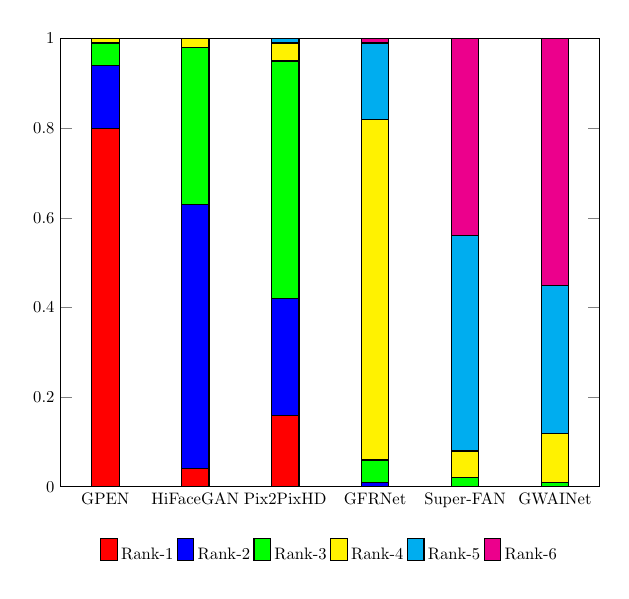
\begin{tikzpicture}[thick,scale=1, every node/.style={scale=0.6}]
   \begin{axis}[
      ybar stacked, ymin=0, ymax=1, 
      symbolic x coords={GPEN, HiFaceGAN, Pix2PixHD, GFRNet, Super-FAN, GWAINet},
      xtick=data,
legend style={draw=none,at={(0.5,-0.1)},anchor=north,legend columns=-1},
      ]

   \addplot [fill=red] coordinates
      {(GPEN,0.8) (HiFaceGAN,0.04) (Pix2PixHD,0.16) (GFRNet,0) (Super-FAN,0) (GWAINet,0)};
   \addplot [fill=blue] coordinates
      {(GPEN,0.14) (HiFaceGAN,0.59) (Pix2PixHD,0.26) (GFRNet,0.01) (Super-FAN,0) (GWAINet,0)};
   \addplot [fill=green] coordinates
      {(GPEN,0.05) (HiFaceGAN,0.35) (Pix2PixHD,0.53) (GFRNet,0.05) (Super-FAN,0.02) (GWAINet,0.01)};
   \addplot [fill=yellow] coordinates
      {(GPEN,0.01) (HiFaceGAN,0.02) (Pix2PixHD,0.04) (GFRNet,0.76) (Super-FAN,0.06) (GWAINet,0.11)};
   \addplot [fill=cyan] coordinates
      {(GPEN,0) (HiFaceGAN,0) (Pix2PixHD,0.01) (GFRNet,0.17) (Super-FAN,0.48) (GWAINet,0.33)};
   \addplot [fill=magenta] coordinates
      {(GPEN,0) (HiFaceGAN,0) (Pix2PixHD,0) (GFRNet,0.01) (Super-FAN,0.44) (GWAINet,0.55)};
   \legend{Rank-1, Rank-2, Rank-3, Rank-4, Rank-5, Rank-6}
   \end{axis}
\end{tikzpicture}
\caption{User study results of different BFR methods.}
\label{fig:ustudy}
\vspace*{-5mm}
\end{figure}

\subsection{Experiments on Images in the Wild}
Finally, we perform experiments on real-world LQ face images, which suffer from complex unknown degradations. We collected  LQ face images from internet for testing. The BFR methods Pix2PixHD \cite{Wang2018Pix2PixHD}, Super-FAN \cite{Bulat2018SuperFAN}, GFRNet \cite{Li2018GFRNet}, GWAInet \cite{Dogan2019Exemplar}, DFDNet \cite{Li2020Restore} and HiFaceGAN \cite{Yang2020HiFaceGANFR} are used in the comparison. Figure~\ref{fig:realcomp} shows the BFR results on three images. One can see that the competing methods fail to restore the facial details. This is mainly because they are trained on synthesized data but have limited generalization capability to the images in the wild. Our method manages to overcome this difficulty by the carefully designed GAN prior embedding and fine-tuning strategies. It not only preserves well the global structure of the face, but also generates realistic details on the face components (e.g., hair, eye, mouth, etc.). Our GPEN can also be successfully used to renovate old photos, as we demonstrated in Figure~\ref{fig:oldphotos}. Please refer to the supplementary material for more results.

Since the commonly used quantitative metrics like PSNR and SSIM do not strongly correlate with human visual perception to image quality, we conduct a user study as a subjective assessment on the performance of our method and the competing methods. The BFR results of GPEN, Pix2PixHD \cite{Wang2018Pix2PixHD}, Super-FAN \cite{Bulat2018SuperFAN}, GFRNet \cite{Li2018GFRNet}, GWAInet \cite{Dogan2019Exemplar}, DFDNet \cite{Li2020Restore} and HiFaceGAN \cite{Yang2020HiFaceGANFR} on  real-world LQ face images collected from internet are presented in a random order to  volunteers for subjective evaluation. The volunteers are asked to rank the six BFR outputs of each input image according to their perceptual quality. Finally, we collect  votes, and the statistics are presented in Figure~\ref{fig:ustudy}. As can be seen, our GPEN method receives much more rank-1 votes than the other state-of-the arts.



\section{Conclusion and Discussion}
We proposed a simple yet effective GAN prior embedded network, namely GPEN, for BFR in the wild. By embedding a pre-trained GAN into a U-shaped DNN as a decoder, and fine-tuning the whole network with artificially degraded face images, our model learned to generate high quality face images from severely degraded ones. Our extensive experiments on synthetic data and real-world images demonstrated that GPEN outperforms the latest state-of-the-arts significantly, restoring clear facial details while retaining properly the image background. The proposed method can also be applied to other tasks such as face inpainting and face colorization. Some preliminary results were provided in the supplementary material. 

The proposed GPEN does not allow multiple HQ images to be generated from a single LQ image in its current form. StyleGAN controls the synthesis via style mixing; however, such an operation may lead to inconsistent image background in GPEN. In the future, we will extend GPEN to allow multiple HQ outputs for a given LQ image. For example, we can use an extra HQ face image as a reference so that different HQ outputs can be generated by GPEN for different reference images. 







{\small
\bibliographystyle{ieee_fullname}
\bibliography{egbib}
}

\end{document}
